\documentclass{polypfe}
\usepackage[a4paper, margin=1in]{geometry}
\usepackage{titlesec}
\usepackage{enumitem}
\usepackage{graphicx}
\usepackage{hyperref}
\usepackage{setspace} 
\usepackage{fancyhdr} 
\usepackage{tabularx}
\usepackage{xcolor}
\usepackage{minitoc}
\usepackage{caption}
\usepackage{longtable}
\usepackage{etoc, soul, lipsum}

\hypersetup{
    colorlinks=true,
    linkcolor=black, 
    citecolor=black,
    filecolor=black,
    urlcolor=black
}

\newcommand\mylocaltableofcontents{%
\begingroup
\renewcommand*{\contentsname}{\textcolor{black}{\textbf{Contents}}\\[-1.0em]\color{black}\rule{\textwidth}{1pt}}
\setcounter{secnumdepth}{3} % Number sections and subsections
\etocsettocdepth{3}

\localtableofcontents
\noindent\rule{\textwidth}{1pt}
\endgroup
}

% Define custom colors using hex codes
\definecolor{blue}{HTML}{0039a6}

% Adjust chapter title formatting
\titleformat{\chapter}[display]
{\normalfont\huge\bfseries}{\chaptertitlename\ \thechapter}{20pt}{\Huge}

% Adjust section title formatting
\titleformat{\section}
{\normalfont\Large\bfseries\color{blue}}{\thesection}{1em}{}

% Adjust subsection title formatting
\titleformat{\subsection}
{\normalfont\large\bfseries\color{blue}}{\thesubsection}{1em}{}

% Adjust subsection title formatting
\titleformat{\subsubsection}
{\normalfont\normalsize\bfseries\color{blue}}{\thesubsubsection}{1em}{}


% Adjust itemize and enumerate formatting
\setlist[itemize]{topsep=0pt, partopsep=0pt, left=1em, label=--}
\setlist[enumerate]{topsep=0pt, partopsep=0pt, left=1em, label=\arabic*.}

\fancyhf{}
\renewcommand{\headrulewidth}{0pt}
\fancyhead[L]{%
    \nouppercase{\leftmark}\\ 
    \rule{\textwidth}{0.4pt} 
}
\fancyfoot[R]{%
    \rule{\textwidth}{0.4pt} \\ 
    \thepage  
}

\fancypagestyle{plain}{
  \fancyhf{}%
  \fancyfoot[R]{%
    \rule{\textwidth}{0.4pt} \\ 
    \thepage  
  }%
  \renewcommand{\headrulewidth}{0pt}
}

\geometry{a4paper, margin=1in}

\setcounter{tocdepth}{3} % Show sections
\setcounter{secnumdepth}{3} % Number sections

\begin{document}

\pagestyle{fancy} 

\pagenumbering{roman}

\tableofcontents

\newpage

\listoffigures

\newpage

\listoftables

\newpage

\pagenumbering{arabic}

\chapter*{General Introduction}

\setstretch{1.5}

In the digital age, email marketing has emerged as a crucial tool for businesses. It provides a platform for businesses to reach out to their customers directly, offering personalized content and promotions that can drive both engagement and sales. This direct line of communication, when coupled with the right messaging, can transform email into one of the most impactful marketing channels. It’s a chance for businesses to speak directly to their customers in their inbox, at a time that is convenient for them.

\vspace{10pt}

Consider the case of Amazon, a global e-commerce giant. Amazon has effectively harnessed the power of email marketing, sending personalized product recommendations and offers to its customers. This strategy significantly enhances customer engagement and drives sales, demonstrating the potential of email marketing. It’s a testament to how understanding customer preferences and tailoring messages accordingly can lead to increased customer loyalty and revenue.

\vspace{10pt}

However, like any other marketing strategy, email marketing comes with its own set of challenges. These include creating engaging content that resonates with the audience, ensuring email deliverability despite the presence of rigorous spam filters, maintaining email lists to ensure they are up-to-date and relevant, and complying with regulations like the General Data Protection Regulation (GDPR). These challenges can make email marketing seem daunting, but they are not invincible.

\vspace{10pt}

To overcome these challenges, businesses are turning to solutions like email builders. These tools provide a seamless and intuitive platform for creating compelling email campaigns. They come equipped with features like drag-and-drop editors, pre-designed templates, and automation tools that make the process of crafting and sending emails a breeze. These tools not only enhance user engagement but also increase brand visibility.

\vspace{10pt}

Moreover, these solutions often come with built-in analytics tools. These tools allow businesses to track key metrics like open rates, click-through rates, and conversion rates. By analyzing these metrics, businesses can gain insights into what’s working and what’s not in their email campaigns, allowing them to continuously optimize their strategies for better results.

\vspace{10pt}

In conclusion, email marketing is a powerful tool for businesses in the digital age. Despite challenges, with the right strategies and tools, it can drive growth and success. Businesses that effectively use email marketing are more likely to succeed. Its influence in the marketing world is significant and will continue to be a dominant force for years to come.


\setstretch{1.5}

\chapter{General presentation and study of the existing}
\mylocaltableofcontents
\newpage

\section*{Introduction}
\addcontentsline{toc}{section}{Introduction}

In this chapter, we will first introduce the host company, Joodlab. Then, we will give an
overview of the general context of our project and explain the working methodology that we
will adopt in our project.

\section{Presentation of the host company}

Joodlab is a technology company that provides the simplest solutions and technical consultations for various companies in different sectors. It was established in Saudi Arabia by a group of experts with multiple competencies in the fields of information technology, artificial intelligence, and information automation. 

\vspace{5pt}

\begin{figure}[ht]
    \centering
    
\includegraphics[width=0.5\linewidth]{Images/logos/joodlab.png}
    \caption{Joodlab logo}
    \label{fig:Joodlab Logo}
\end{figure}




\section{Project context}

In this part, we will present the main issue, a study of the existing solutions, our project’s
goals as well as the different steps of the project.

\subsection{Main issue}
The primary challenge in the field of email marketing is the creation and management of effective email campaigns. This involves several aspects:

\begin{itemize}
\item \textbf{Email Creation:} The process of creating an email should be intuitive and efficient. Currently, many tools require knowledge of HTML and CSS for customization, which can be a barrier for non-technical users.

\item \textbf{Customization:} Users should be able to easily customize their emails to fit their brand and message. This includes the ability to change styles, add elements, and adjust layouts.

\item \textbf{Campaign Management:} Managing an email campaign involves sending out emails, scheduling them, and segmenting the audience. These tasks should be easy to perform and manage within the tool.

\item \textbf{Tracking:} Once an email campaign is sent out, it's crucial to track its performance. This includes open rates, click-through rates, and conversions. The tool should provide comprehensive tracking and analytics.

\item \textbf{Usability:} The tool should be user-friendly, with a clean interface and clear instructions. It should cater to both beginners and advanced users, offering simplicity without compromising on features.
\end{itemize}

The lack of a tool that effectively addresses all these aspects is the main issue we aim to solve with our SaaS email marketing application.



\subsection{Analysis of the existing solutions}

\subsubsection{HubSpot}

\begin{figure}[ht]
    \centering
    
\includegraphics[width=0.5\linewidth]{Images/logos/hubspot.png}
    \caption{HubSpot logo}
    \label{fig:HubSpot Logo}
\end{figure}

While HubSpot is a comprehensive platform for email marketing, it has several limitations that can affect its usability and effectiveness:

\vspace{10pt}

\begin{itemize}
\item \textbf{Limited Free Version:} The free version of HubSpot’s email marketing tool is limited. You can only send 2,000 emails per month. Additionally, you cannot connect to a custom email sending domain. This means your emails will show “via HubSpot” in the sender area and the footer of your email will have a HubSpot logo.

\item \textbf{Sending Limits:} HubSpot’s send limits vary based on each email provider’s limit. For instance, Gmail Free allows 350 emails per day, Google Apps, Office 365, Exchange inbox, and Generic inbox allow 1000 emails per day.

\item \textbf{CRM Limitations:} There are major limitations for sales functionality in the free CRM. These include only 15 minutes of calling per user, per month, no inbound calling, HubSpot branding on emails, only one sales pipeline, and no email automation.
\end{itemize}

\subsubsection{Constant Contact}

\begin{figure}[ht]
    \centering
    
\includegraphics[width=0.5\linewidth]{Images/logos/Constant-Contact.png}
    \caption{Constant Contact logo}
    \label{Constant Contact Logo}
\end{figure}

Constant Contact, despite its popularity, also has its drawbacks:

\vspace{10pt}

\begin{itemize}
\item \textbf{Inflexible Email Editor:} The email editor is not as flexible or intuitive as users might prefer, which can make the process of creating emails more time-consuming and less efficient.
\item \textbf{Limited Tracking Features:} The tracking features, while useful, do not offer as much depth as other tools. This can limit user's ability to fully understand and optimize their email campaigns.
\end{itemize}

\vspace{10pt}

In summary, both HubSpot and Constant Contact have significant limitations that can hinder the efficiency and effectiveness of email marketing. Our proposed solution aims to address these limitations by offering a more intuitive and flexible email builder, more customizable design options, and more accessible yet comprehensive campaign tracking.


\subsection{Overview of the Suggested Solution}
Our proposed solution is a Software as a Service (SaaS) application designed to revolutionize email marketing. The key features of our solution include:

\vspace{10pt}

\begin{itemize}
\item \textbf{Drag-and-Drop Email Builder:} Our solution includes a user-friendly drag-and-drop email builder. This allows users to easily create professional and personalized emails without needing any technical skills. The builder includes a variety of elements that can be added to an email, such as text boxes, images, buttons, and more.

\item \textbf{Customizable Elements:} Each element in the email builder is fully customizable. Users can change the style, size, color, and other properties of these elements to fit their brand and message. This level of customization allows for the creation of unique and engaging emails.

\item \textbf{Email Sending and Campaign Creation:} Our solution makes it easy to send out emails and create marketing campaigns. Users can schedule emails to be sent at specific times, segment their audience to target specific groups, and automate their email marketing process.

\item \textbf{Campaign Tracking:} To help users measure the success of their email marketing efforts, our solution includes comprehensive campaign tracking features. Users can track open rates, click-through rates, and conversions, and use this data to optimize their future campaigns.

\item \textbf{User-Friendly Interface:} Our solution features a clean and intuitive interface, making it easy for users to navigate and use the various features. This ensures a smooth user experience, regardless of the user's technical skills.

\end{itemize}

\vspace{10pt}

\begin{table}[ht]
\centering
\begin{tabularx}{\textwidth}{|X|c|c|c|}
\hline
\textbf{Feature} & \textbf{HubSpot} & \textbf{Constant Contact} & \textbf{Our Tool} \\
\hline
Tracking & Yes & Yes & Yes \\
\hline
Campaign Management & Yes & Yes & Yes \\
\hline
Email Builder & Limited & Limited & Yes \\
\hline
Customization & Limited & Limited & Yes \\
\hline
\end{tabularx}
\caption{Comparison of HubSpot, Constant Contact, and our Email Marketing Tool}
\label{tab:comparison table}
\end{table}

\vspace{10pt}

In summary, our SaaS application aims to provide a more intuitive, efficient, and effective approach to email marketing. By addressing the limitations of existing solutions, we believe our tool can significantly improve the email marketing process for businesses of all sizes.



\section{Adopted Methodology}

In this section, we will discuss the methodology adopted for the development of our SaaS email marketing application.

\subsection{Methodology Choice}

For this project, we have chosen to adopt the SCRUM methodology. This decision was made due to several reasons. Firstly, SCRUM is an agile development methodology which allows for rapid iteration and flexibility. This is particularly important for our project as it allows us to quickly adapt to changes and continuously improve our product based on user feedback. Secondly, SCRUM promotes close collaboration among team members which helps to ensure that everyone is on the same page and working towards the same goals.

\subsection{Introduction to SCRUM}

\begin{figure}[ht]
    \centering
    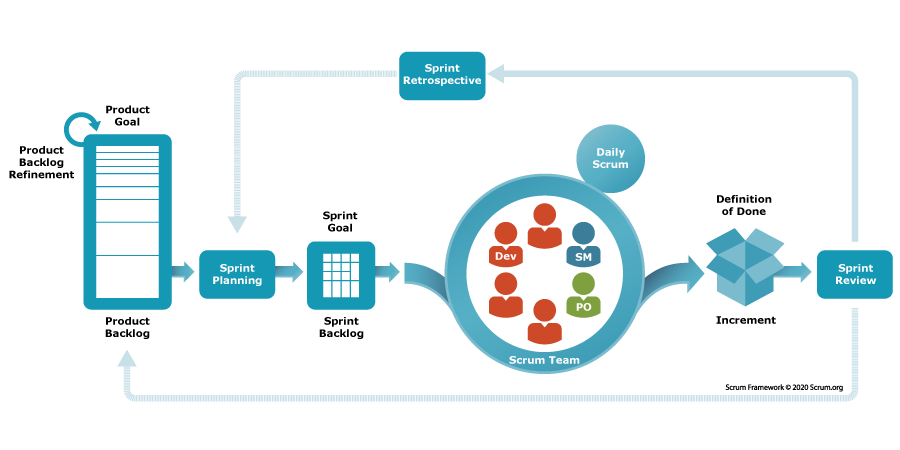
\includegraphics[width=0.6\linewidth]{Images//images/scrum.png}
    \caption{Life-cycle of the Scrum method}
    \label{fig:Life-cycle of the Scrum method}
\end{figure}

SCRUM is a framework for agile development. It is designed to add energy, focus, clarity, and transparency to project planning and implementation. At its core, SCRUM is about empowering a self-managing team to deliver, and it uses iterative, incremental practices to increase productivity and optimize predictability. In the context of our project, SCRUM provides a structured approach to managing the complex task of developing a new software product.

\subsection{SCRUM Roles}
Within the SCRUM framework, there are three key roles: the Product Owner, the Scrum Master, and the Development Team.

\vspace{10pt}

\begin{itemize}
\item \textbf{Product Owner:} The Product Owner is responsible for maximizing the value of the product resulting from the work of the Development Team. They manage the Product Backlog and are the sole person responsible for its content, availability, and ordering.

\item \textbf{Scrum Master:} The Scrum Master is responsible for promoting and supporting SCRUM. They do this by helping everyone understand SCRUM theory, practices, rules, and values. The Scrum Master serves the team by removing impediments to the team's progress.

\item \textbf{Development Team:} The Development Team is responsible for delivering potentially shippable increments of the product at the end of each Sprint. The team is self-organizing, cross-functional, and has all the skills necessary to create a product Increment.
\end{itemize}

\subsection{Product Backlog}
The Product Backlog is a list of features, functions, requirements, enhancements, and fixes that constitute the changes to be made to the product in future releases. It is the single source of requirements for any changes to be made to the product. The Product Owner is responsible for the Product Backlog, including its content, availability, and ordering.

\vspace{10pt}

\begin{itemize}
\item \textbf{Content:} The Product Backlog lists all features, functions, requirements, enhancements, and fixes that need to be made to the product. Each item in the backlog is expressed as a user story which provides a clear understanding of the requirement from an end-user perspective.
\item \textbf{Availability:} The Product Backlog is a living document that is available to all stakeholders. This ensures transparency and allows everyone involved in the project to understand the direction of the product and the work to be done.
\item \textbf{Ordering:} The items in the Product Backlog are ordered by the Product Owner based on their value, risk, priority, and necessity. This helps the Development Team to understand the work items' relative priority.
\end{itemize}

\subsection{The Sprint}
A Sprint is a time-boxed period during which specific work has to be completed and made ready for review. Sprints typically last between one week to one month. Here are the key aspects of a Sprint:

\vspace{10pt}

\begin{itemize}
\item \textbf{Sprint Planning:} At the start of the Sprint, the team holds a planning meeting to decide what work will be accomplished during the Sprint. The Product Owner identifies the items in the Product Backlog that he or she wants completed (the Sprint Goal) and the team decides how much of this they can commit to complete during the next Sprint.
\item \textbf{Daily Scrum:} Each day during the Sprint, the team holds a daily scrum meeting to discuss progress and plan for the day. This is not a problem-solving or issue resolution meeting. Instead, it is a chance for the team to inspect their progress towards the Sprint Goal and adjust their plan as necessary.
\item \textbf{Sprint Review:} At the end of the Sprint, the team holds a Sprint Review to inspect the Increment and adapt the Product Backlog if needed. During the Sprint Review, the Scrum Team and stakeholders collaborate about what was done in the Sprint.
\item \textbf{Sprint Retrospective:} After the Sprint Review and prior to the next Sprint Planning, the team holds a Sprint Retrospective. During this meeting, the team discusses what went well, what didn't, and how they can make improvements for the next Sprint.
\end{itemize}



\section*{Conclusion}
\addcontentsline{toc}{section}{Conclusion}

In conclusion, our SaaS email marketing tool, with its user-friendly drag-and-drop email builder and customizable elements, aims to address the limitations of existing solutions such as HubSpot. By adopting the SCRUM methodology, we ensure a flexible and iterative development process, allowing for continuous product improvement based on user feedback.

\vspace{5pt}

The SCRUM roles of Product Owner, Scrum Master, and Development Team will work collaboratively throughout the development process. The use of a Product Backlog and Sprints will effectively manage tasks and progress.

\vspace{5pt}

Overall, we believe our approach will lead to the successful development of a tool that significantly improves the email marketing process, providing value to our users and setting a new industry standard.




\chapter{Requirements and specifications}
\mylocaltableofcontents
\newpage

\section*{Introduction}
\addcontentsline{toc}{section}{Introduction}

This chapter starts with a brief introduction to the project. We’ll then identify the key players and requirements. Next, we’ll model the functional requirements and plan the product backlog and sprints. Finally, we’ll discuss the development environment for the project.
\section{Email marketing tool Requirements}

This section outlines the requirements for an email marketing tool. The tool is designed to meet the needs of various actors. The requirements are divided into functional and non-functional requirements, providing a comprehensive overview of what the system is expected to do and the standards it should adhere to.

\subsection{Identification of the actors}
The system will interact with the following actors:
\begin{itemize}
\item \textbf{New User}: A person who has not registered an account yet.
\item \textbf{User}: A person who has registered an account and can log in.
\item \textbf{Administrator}: A user who has created an organization and manages it.
\end{itemize}

\subsection{Functional Requirements}

\subsubsection{New Users}
\begin{itemize}
    \item \textbf{Account Registration}
\end{itemize}

\subsubsection{Users}
\begin{itemize}
\item \textbf{Account Login}
\item \textbf{Organization Creation}
\item \textbf{Organization List View}
\item \textbf{Email Template Creation}
\item \textbf{Email Template Editing}
\item \textbf{Email Template List View}
\item \textbf{Email Template Search}
\item \textbf{Draft Management}
\item \textbf{Email Sending}
\item \textbf{Sent Email History}
\item \textbf{Campaign Creation}
\item \textbf{Campaign Management}
\item \textbf{Campaign List View}
\item \textbf{Campaign Insights}
\item \textbf{Media Cloud}
\end{itemize}

\subsubsection{Administrators}
\begin{itemize}
\item \textbf{User Deactivation/Removal}
\item \textbf{User Addition and Role Assignment}
\item \textbf{Role Management}
\end{itemize}


\subsection{Non-functional requirements}
The non-functional requirements of the system are as follows:
\begin{itemize}
\item \textbf{Security}: The system should securely store user credentials and personal information. It should also provide secure access control mechanisms.
\item \textbf{Usability}: The system should be user-friendly, allowing users to easily navigate and manage their organizations and email templates.
\item \textbf{Performance}: The system should provide fast and efficient access to the shared work within an organization.
\item \textbf{Reliability}: The system should reliably deliver emails and track their status and timestamp.
\item \textbf{Scalability}: The system should be able to handle a large number of users, organizations, and email templates without performance degradation.
\item \textbf{Maintainability}: The system should be easy to update and maintain, allowing for the addition of new features and updates to existing ones.
\end{itemize}

\section{Work Environment}

This section outlines the work environment for the project, including the hardware environment, development environment, and software environment.

\subsection{Software Environment}

In our project, we used the following tools:

\subsubsection*{Visual Studio Code}
\begin{center}

\includegraphics[width=0.15\textwidth]{Images/logos/vscode.png}
\captionof{figure}{Visual Studio Code logo}
\label{fig:vscode}
\end{center}
The development environment for this project is a combination of the software tools mentioned in the Software Environment section. Each tool plays a crucial role in different aspects of the development process \cite{vscode}.

\clearpage

\subsubsection*{GitLab}
\begin{center}

\includegraphics[width=0.2\textwidth]{Images/logos/gitlab-logo-500.png}
\captionof{figure}{GitLab logo}
\label{fig:gitlab}
\end{center}
GitLab serves as the remote repository for code hosting and versioning. It also provides a platform for creating CI/CD pipelines, facilitating continuous integration and deployment of the project \cite{gitlab}.

\subsubsection*{Notion}
\begin{center}

\includegraphics[width=0.2\textwidth]{Images/logos/62cc159e150d5de9a3dad5ec.png}
\captionof{figure}{Notion logo}
\label{fig:notion}
\end{center}
Notion serves as the central hub for project management. It is used for task tracking, documentation, and collaboration, providing a unified workspace for all project-related information and tasks \cite{notion}.

\subsubsection*{Postman}
\begin{center}

\includegraphics[width=0.2\textwidth]{Images/logos/62cc1b6b150d5de9a3dad5f9.png}
\captionof{figure}{Postman logo}
\label{fig:postman}
\end{center}
Postman is used for testing and debugging APIs. It simplifies the process of building, testing, and modifying APIs, making it an essential tool for backend development \cite{postman}.

\clearpage

\subsubsection*{DBeaver}
\begin{center}

\includegraphics[width=0.2\textwidth]{Images/logos/DBeaver_logo.png}
\captionof{figure}{DBeaver logo}
\label{fig:dbeaver}
\end{center}
DBeaver is used for database management and interaction. It supports a wide range of databases and provides a user-friendly interface for managing database schemas, running SQL queries, and performing other database-related tasks \cite{dbeaver}.

\subsubsection*{Docker Desktop}
\begin{center}

\includegraphics[width=0.2\textwidth]{Images/logos/docker-mark-blue.png}
\captionof{figure}{Docker Desktop logo}
\label{fig:docker}
\end{center}
Docker Desktop is used to containerize the services. It allows for the packaging and distribution of applications in a manner that is independent of the host operating system, ensuring consistent operation across different computing environments \cite{docker}.

\subsubsection*{Git}
\begin{center}

\includegraphics[width=0.2\textwidth]{Images/logos/Git-Icon-1788C.png}
\captionof{figure}{Git logo}
\label{fig:git}
\end{center}
Git is used for version control, allowing for efficient tracking and management of changes to the project codebase. It is an essential tool for collaborative development \cite{git}.

\subsubsection*{Brevo}
\begin{center}

\includegraphics[width=0.2\textwidth]{Images/logos/Brevo-Logo.png}
\captionof{figure}{Brevo logo}
\label{fig:brevo}
\end{center}
Brevo was utilized for transactional webhook and email services, providing reliable communication channels for real-time updates and notifications within the application \cite{brevo}.

\subsection{Development Environment}

\subsubsection*{Node.js}
\begin{center}

\includegraphics[width=0.15\textwidth]{Images/logos/node.png}
\captionof{figure}{Node.js logo}
\label{fig:nodejs}
\end{center}
Node.js is a JavaScript runtime built on Chrome’s V8 JavaScript engine. It’s used for building scalable network applications and executing JavaScript code server-side \cite{node}.

\subsubsection*{TypeScript}
\begin{center}

\includegraphics[width=0.15\textwidth]{Images/logos/ts-lettermark-blue.png}
\captionof{figure}{TypeScript logo}
\label{fig:typescript}
\end{center}
TypeScript is a typed superset of JavaScript that adds static types. It helps to write more robust code and maintain a cleaner and more consistent codebase. It’s used in this project along with Vue 3 for building user interfaces \cite{typescript}.

\subsubsection*{Vue 3}
\begin{center}

\includegraphics[width=0.15\textwidth]{Images/logos/vue.png}
\captionof{figure}{Vue 3 logo}
\label{fig:vue3}
\end{center}
Vue 3 is the latest version of Vue.js, a progressive JavaScript framework for building user interfaces \cite{vue3}.

\clearpage

\subsubsection*{Tailwind CSS}
\begin{center}

\includegraphics[width=0.15\textwidth]{Images/logos/tailwind.png}
\captionof{figure}{Tailwind CSS logo}
\label{fig:tailwind}
\end{center}
Tailwind CSS is a utility-first CSS framework for rapidly building custom user interfaces. It provides low-level utility classes that let you build completely custom designs without ever leaving your HTML \cite{tailwind}.

\subsubsection*{Fastify}
\begin{center}

\includegraphics[width=0.15\textwidth]{Images/logos/fastify.png}
\captionof{figure}{Fastify logo}
\label{fig:fastify}
\end{center}
Fastify is a web framework highly focused on providing the best developer experience with the least overhead and a powerful plugin architecture. It is used for building efficient and scalable Node.js web applications \cite{fastify}.

\subsubsection*{MJML}
\begin{center}

\includegraphics[width=0.15\textwidth]{Images/logos/file-type-mjml.512x453.png}
\captionof{figure}{MJML logo}
\label{fig:MJML}
\end{center}
MJML is a markup language designed to simplify the process of coding responsive emails. It provides a semantic syntax and a library of standard components, making it easier to build custom email templates that are responsive and compatible with various email clients \cite{mjml}.

\clearpage

\subsubsection*{Turborepo}
\begin{center}

\includegraphics[width=0.15\textwidth]{Images/logos/turbopack-logotype-light-background.png}
\captionof{figure}{Turborepo logo}
\label{fig:turborepo}
\end{center}
Turborepo is a high-performance build system for JavaScript and TypeScript codebases. It provides features like incremental builds, parallel execution, and remote caching. It’s designed for monorepos, improving build times and facilitating efficient project management \cite{turborepo}.

\subsubsection*{Prisma}
\begin{center}

\includegraphics[width=0.15\textwidth]{Images/logos/Prisma.png}
\captionof{figure}{Prisma logo}
\label{fig:prisma}
\end{center}
Prisma is an open-source database toolkit. It replaces traditional ORMs and makes database access easy with an auto-generated and type-safe query builder that’s tailored to your database schema \cite{prisma}.

\subsubsection*{Swagger}
\begin{center}

\includegraphics[width=0.15\textwidth]{Images/logos/Swagger-logo.png}
\captionof{figure}{Swagger logo}
\label{fig:swagger}
\end{center}
Swagger is an open-source software framework backed by a large ecosystem of tools that helps developers design, build, document, and consume RESTful web services. It’s used in this project for API design and documentation \cite{swagger}.
\section{Project Management with Scrum}

This section outlines the key aspects of project management with Scrum including the product backlog, use case diagram, sprint planning, and interface prototyping.

\subsection{Backlog Features}

\begin{longtable}{|c|p{0.83\textwidth}|c|}
	\hline
	\textbf{ID} & \textbf{Description} & \textbf{Effort} \\
	\hline
	1           & Register for an account with a password and email to access the system. & Low \\
	\hline
	2           & Log in to the account using email and password for secure access. & Low \\
	\hline
	3           & Reset the password via email in case of forgetting it. & Low \\
	\hline
	4           & Create a new organization with a unique name and become its administrator to manage users and templates. & High \\
	\hline
	5           & View a list of all organizations to navigate and manage them. & Medium \\
	\hline
	6           & Access shared work (templates, campaigns, media) within the organization for effective collaboration. & High \\
	\hline
	7           & Deactivate or remove users from the organization for security and access control. & Medium \\
	\hline
	8           & Add users to the organization and assign specific roles for access control. & High \\
	\hline
	9           & View and manage user roles within the organization. & Medium \\
	\hline
	10          & Create new email templates for sending emails. & High \\
	\hline
	11          & Edit and update email templates to keep information accurate. & Medium \\
	\hline
	12          & View a list of all email templates for easy management. & Low \\
	\hline
	13          & Create and manage email template drafts before finalizing and sending. & High \\
	\hline
	14          & Create and publish campaigns using selected templates to organize and track marketing efforts.. & High \\
	\hline
	15          & View a history of published campaigns for reference. & Low \\
	\hline
	16          & Generate reports for campaign analysis and informed decision-making. & High \\
	\hline
\end{longtable}

\clearpage
\subsection{Global Use Case Diagram}
Figure \ref{fig:Global Use Case Diagram} offer us a global overview by presenting a visual description of the functional
behaviour of our tool. This diagram sums up the interactions among the actors and the
diverse use cases within the system.

\begin{figure}[ht]
	\centering
	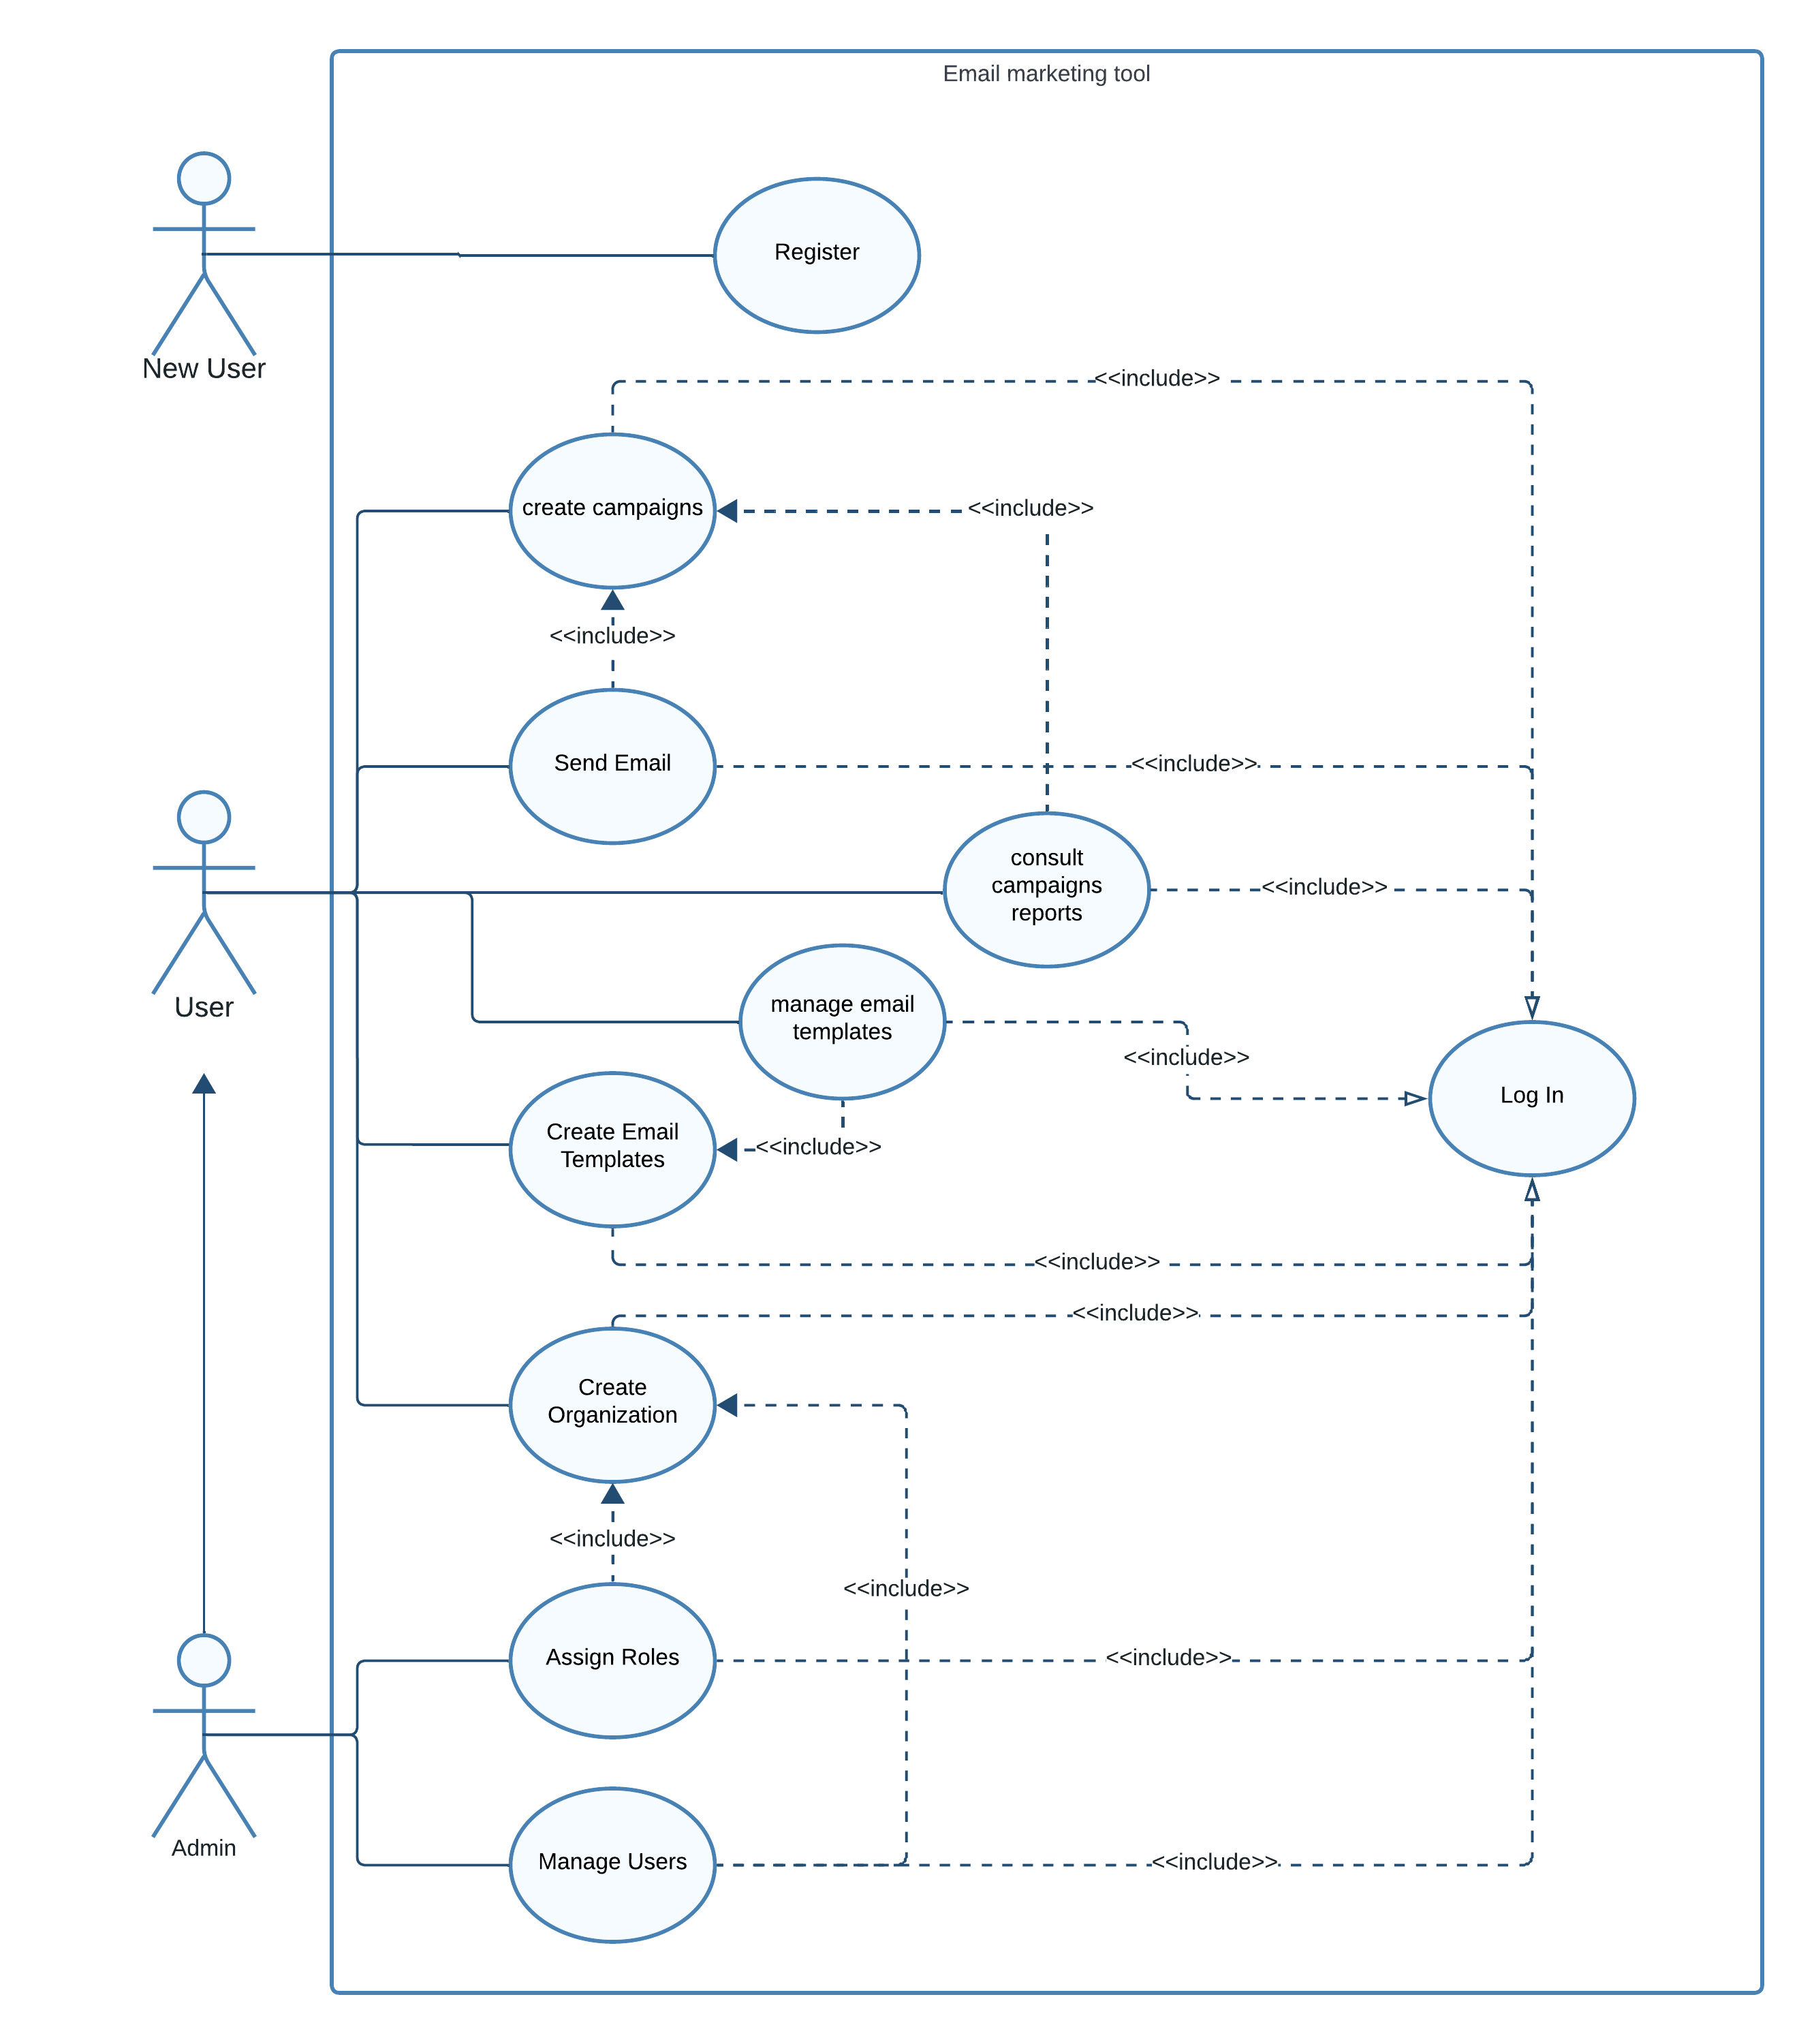
\includegraphics[width=\linewidth]{Images//images/global use case diag.png}
	\caption{Global Use Case Diagram}
	\label{fig:Global Use Case Diagram}
\end{figure}

\newpage

\subsection{Sprint Planning}

Figure \ref{fig:Sprint Planning} outlines our project's sprint planning. Each sprint had specific goals and durations. The initial phase was for learning the necessary tools. \textbf{Sprint 1} focused on building the email builder and creating and managing campaigns and audience. \textbf{Sprint 2} worked on CI/CD pipelines and deployed the application. \textbf{Sprint 3} implemented email tracking functionality, and conducted final testing and bug fixing across all features. This structured approach ensured thorough development and testing of each feature. As a result, all planned features were successfully implemented and thoroughly tested within the project timeline.

\begin{figure}[ht]
	\centering
	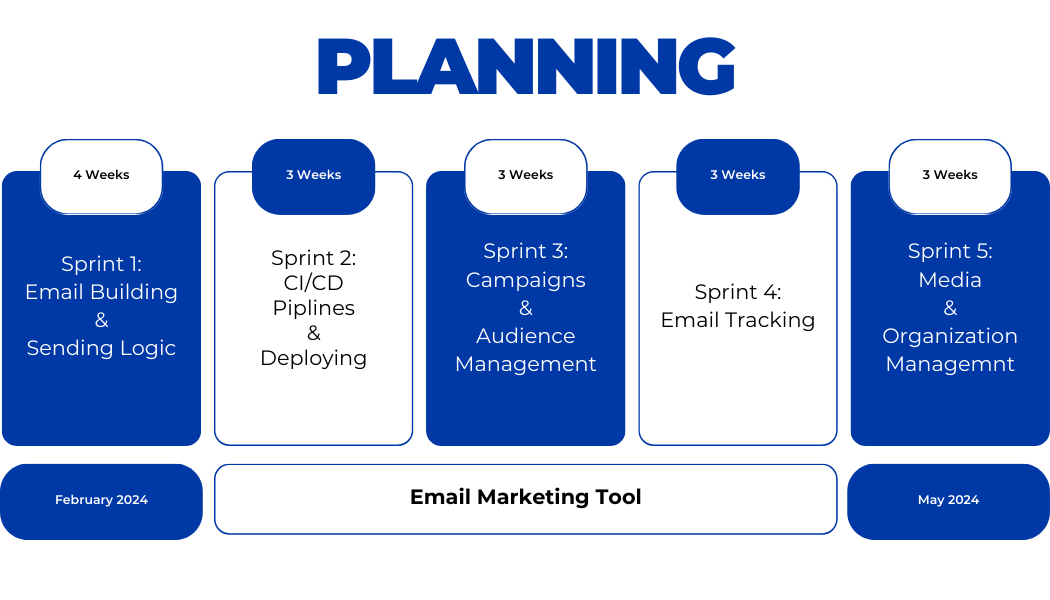
\includegraphics[width=\linewidth]{Images//images/planning.png}
	\caption{Sprint Planning}
	\label{fig:Sprint Planning}
\end{figure}

%\clearpage

\section{General Architecture of the Application}

This section outlines the general architecture of the application. It includes the physical architecture and the operation of the architecture.

\subsection{Physical Architecture}

\begin{figure}[ht]
	\centering
	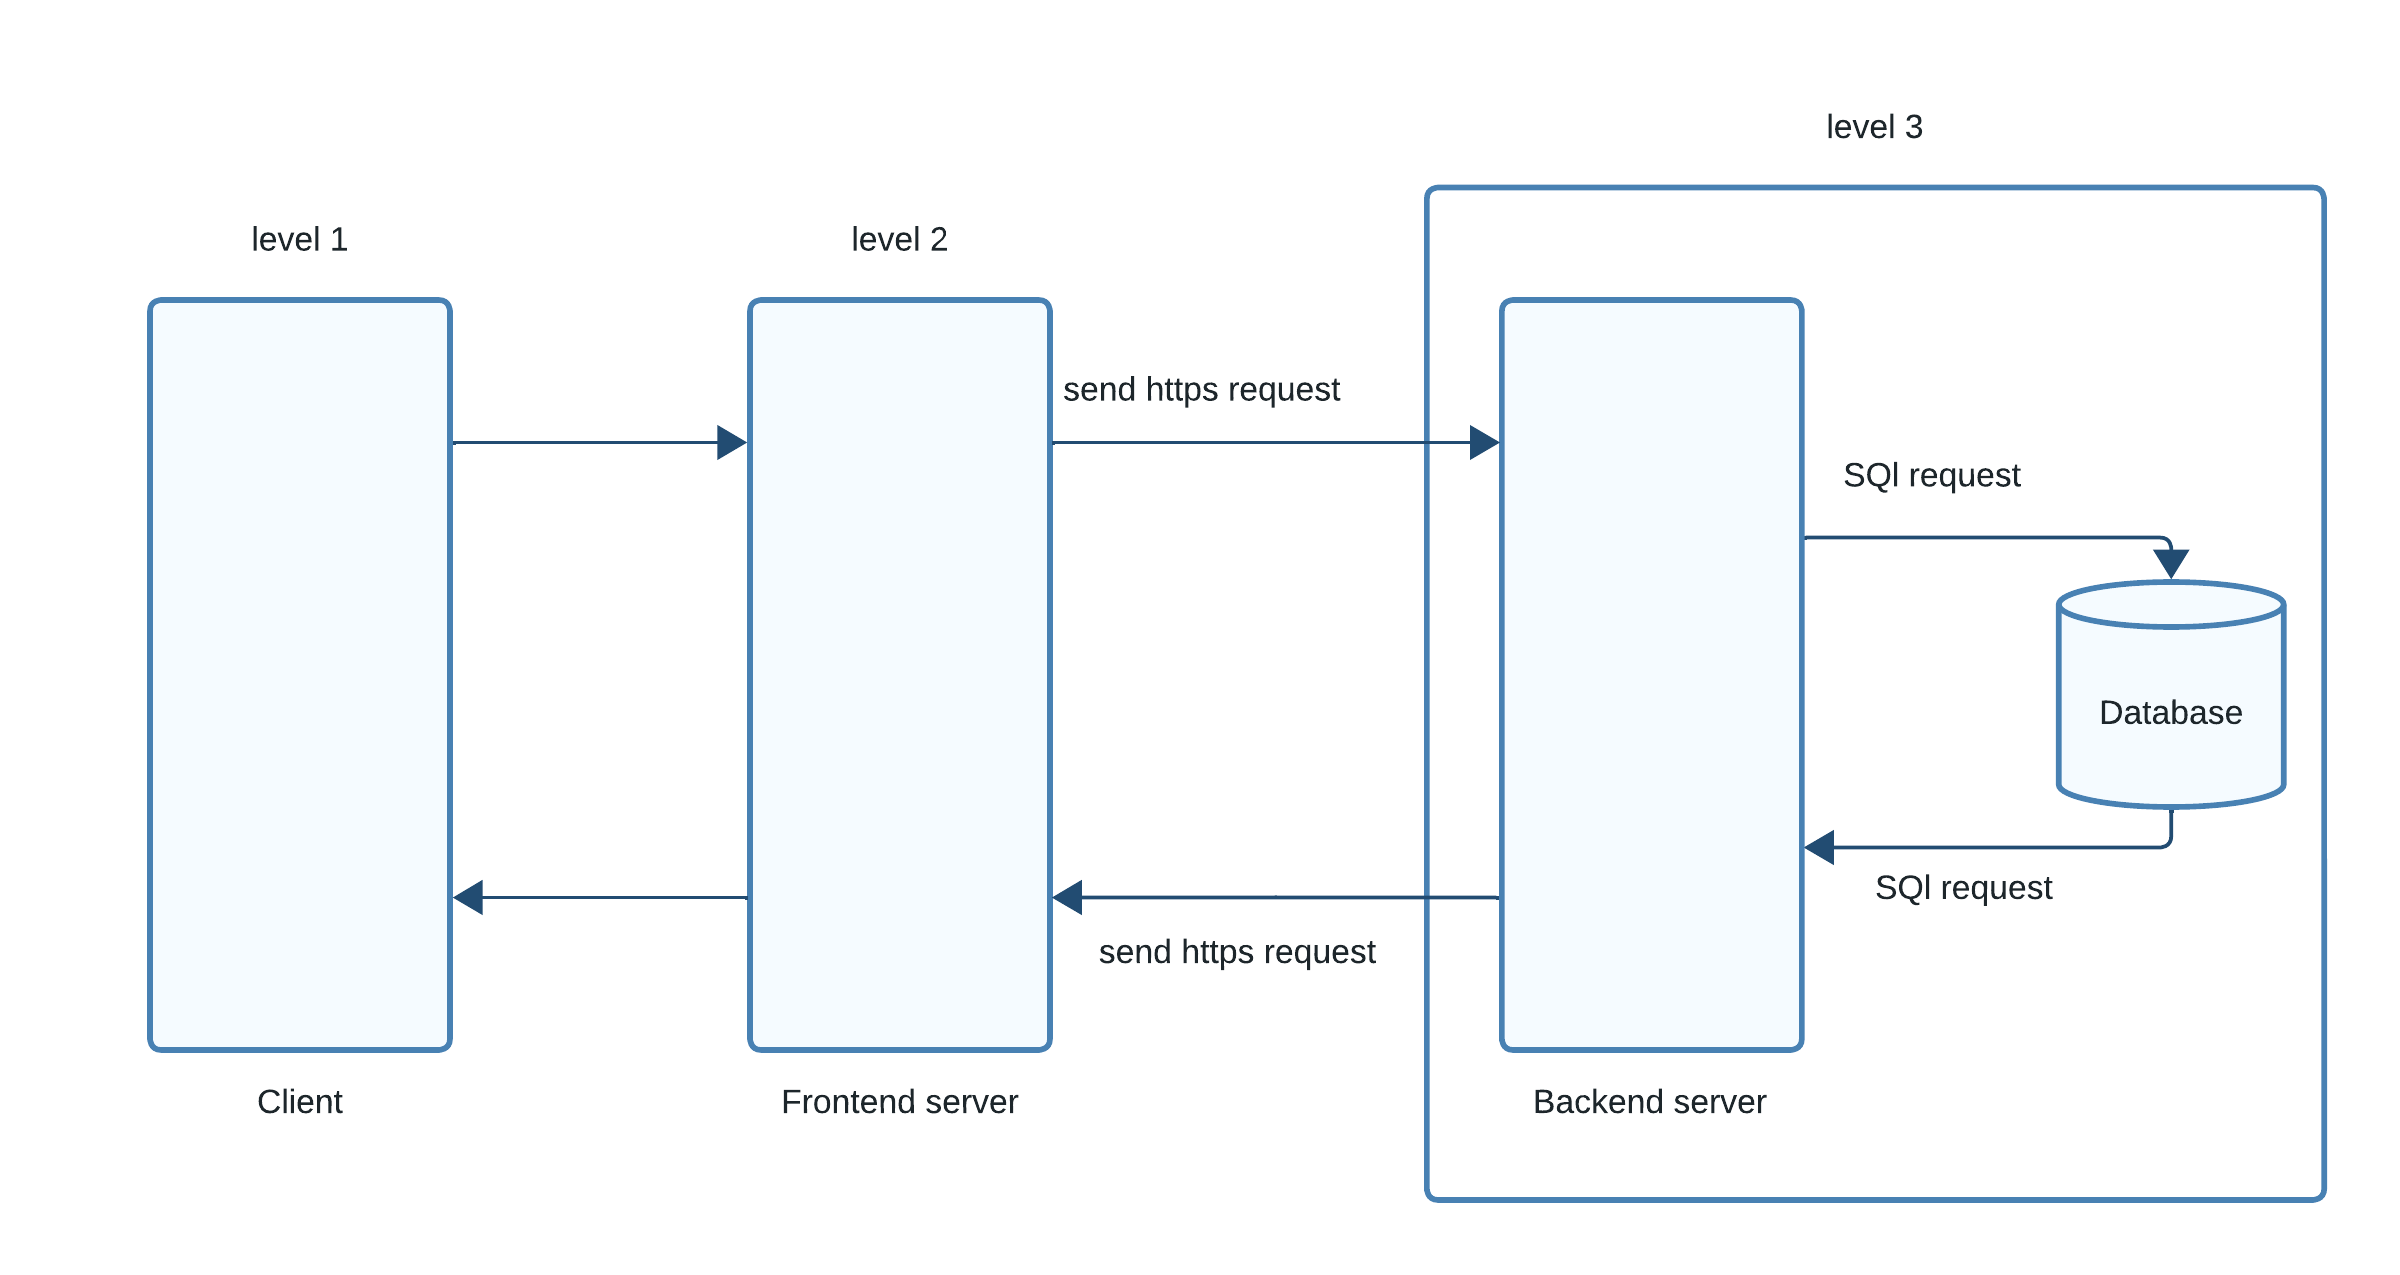
\includegraphics[width=\linewidth]{Images//images/3-tier architecture.png}
	\caption{Global Use Case Diagram}
	\label{fig:Global Use Case Diagram}
\end{figure}

In the physical architecture, I followed the 3-tier architecture:

\begin{itemize}
	\item Level 1 is the Client (Presentation Tier): This is where the user interacts with the system. It could be any user interface like a web page, desktop application, or mobile app.
	\item Level 2 is the Front Server (Application Tier): This is where all the business logic resides. It processes client requests, manages business rules, and controls application functionality.
	\item Level 3 is the Back Server and Database (Data Tier): This is where data is stored and retrieved. It includes the database management system and the servers that manage it.
\end{itemize}

\clearpage
\subsection{Logical Architecture}

\begin{figure}[ht]
	\centering
	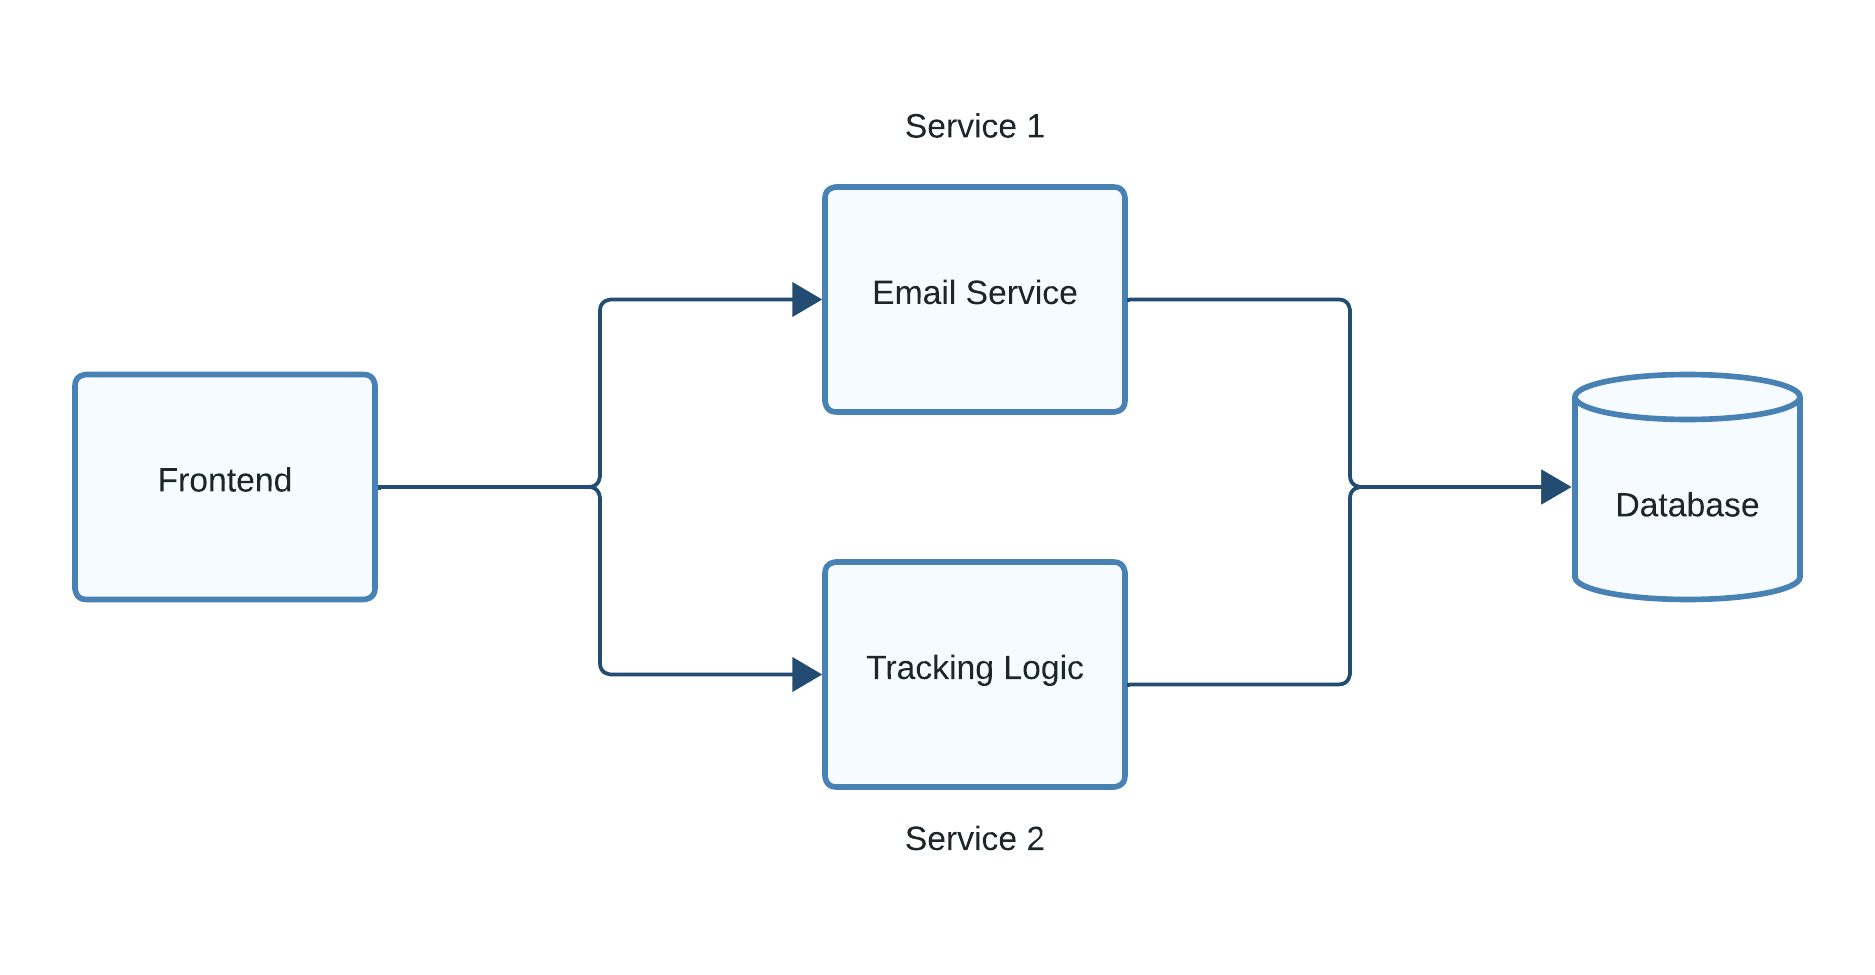
\includegraphics[width=\linewidth]{Images//images/Microservices architechture.png}
	\caption{Global Use Case Diagram}
	\label{fig:Global Use Case Diagram}
\end{figure}
The logical architecture of our email marketing tool consists of several interconnected components:

\begin{itemize}
	\item \textbf{Frontend}:
	      \begin{itemize}
		      \item This component represents the user-facing part of our application.
		      \item It is deployed on Vercel, a platform for hosting frontend applications.
		      \item Users interact with the frontend to create and manage email campaigns, templates, and other settings.
	      \end{itemize}

	\item \textbf{Email Building and Sending Service}:
	      \begin{itemize}
		      \item Responsible for email composition, rendering, and sending logic.
		      \item Communicates with the frontend to receive email content and recipient lists.
		      \item Handles the process of sending emails to recipients.
		      \item It is deployed on Azure.
	      \end{itemize}

	\item \textbf{Tracking Service}:
	      \begin{itemize}
		      \item Tracks email campaign performance metrics.
		      \item Collects data on email opens, clicks, and other relevant events.
		      \item Stores tracking data for analytics and reporting purposes.
              \item It is deployed on Azure.
	      \end{itemize}

	\item \textbf{Database}:
	      \begin{itemize}
		      \item Hosts our Campaign-related data.
		      \item Contains three main tables:
		            \begin{itemize}
			            \item \textbf{Email Campaigns Data}: Stores email content, and recipient information.
			            \item \textbf{Email Template}: Stores built email templates
			            \item \textbf{Tracking Data}: Stores tracking events (e.g., opens, clicks) associated with email campaigns.
		            \end{itemize}
	      \end{itemize}
\end{itemize}

%\section{Deployment Diagram}

Provide a deployment diagram that shows how your application will be deployed in a live environment. This could include servers, databases, and the connections between them.
\section*{Conclusion}
\addcontentsline{toc}{section}{Conclusion}

In this chapter, we identified the functional and non-functional requirements of our applica-
tion. Then, we aligned scrum to our project. Finally, we chose our working environment.

\end{document}
